\documentclass[11pt]{article}
\usepackage[margin=1in]{geometry}
\usepackage[T1]{fontenc}
\usepackage[utf8]{inputenc}
\usepackage{lmodern}
\usepackage{microtype}
\usepackage{graphicx}
\usepackage{booktabs}
\usepackage{enumitem}
\usepackage{hyperref}
\usepackage{xcolor}

\hypersetup{
  colorlinks=true,
  linkcolor=blue!50!black,
  urlcolor=blue!50!black,
  citecolor=blue!50!black
}

\title{AlphaGateau for Breakthrough:\\A Graph-Based AlphaZero-Style Agent With Cross-Board Transfer}
\author{
  Athmane Benarous \and
  Farooq Khan \and
  Andrew Saffar
}
\date{}

\begin{document}
\maketitle

\begin{abstract}
We adapt AlphaGateau, a graph-neural reinterpretation of AlphaZero, from chess to the abstract strategy game Breakthrough. Our implementation introduces a custom JAX Breakthrough environment, a board-size-invariant graph encoder, an AlphaGateau-style GNN policy/value network, and a simpler AlphaZero-style CNN baseline on 8x8 boards. The main experimental question is whether graph structure helps both direct learning on 8x8 Breakthrough and transfer from 5x5 pretraining to 8x8 fine-tuning. The repository supports the full planned training schedule, automated evaluation, Elo estimation with weighted least squares, figure generation, and a Slurm-native experiment DAG for the McGill department GPU allocation.
\end{abstract}

\section{Introduction}

Breakthrough is a clean adversarial benchmark for reinforcement learning because its rules are simple while its tactics are highly local and geometry-dependent. Every move is a one-step forward advance or diagonal advance, and winning requires either reaching the opponent's back rank or otherwise forcing a decisive terminal state. This makes the game a natural target for graph-based state representations: legal moves define directed relationships between squares, and those relationships are more structured than a raw image-like grid.

AlphaZero-style systems traditionally use convolutional networks over board tensors, but AlphaGateau argues that graph representations can encode board games more naturally while also improving parameter sharing across board sizes. Our project tests that hypothesis in Breakthrough by re-implementing the full self-play, MCTS, policy-value learning loop on top of a custom environment rather than the chess-specific PGX stack used by the upstream AlphaGateau code.

\section{Background}

AlphaZero combines self-play reinforcement learning with Monte Carlo Tree Search (MCTS). A neural network predicts both a policy over legal actions and a scalar state value, and MCTS uses those predictions to improve search-time action selection. The search output becomes the policy target for training, while the eventual game outcome becomes the value target.

AlphaGateau replaces convolutional layers with a graph neural network that updates node and edge features jointly. This matters for Breakthrough because the game is naturally described by squares and move relations. Unlike a fixed 8x8 tensor model, a graph model can preserve a consistent feature schema while the number of squares changes from 5x5 to 8x8. That property is central to our transfer experiment.

\section{Methodology}

\subsection{Environment}

We implemented a custom \texttt{BreakthroughEnv(board\_size)} in JAX with the state fields needed by the AlphaZero-style pipeline: board tensor, canonical observation, legal action mask, current player, rewards, and terminal flag. The action space is fixed to
\[
\texttt{action = from\_square * 3 + move\_type}
\]
where \texttt{move\_type} is one of \{\texttt{forward}, \texttt{diag\_left}, \texttt{diag\_right}\} in the current player's canonical perspective. The environment rotates the board into a canonical view so the side to move always advances in the same direction. This keeps both the graph encoder and the MCTS model interface board-size agnostic.

\subsection{State Encodings}

The CNN baseline consumes a canonical tensor observation with channels for self pieces, opponent pieces, and empty squares. The GNN uses a graph with one node per square and directed move edges for both players.

Node features are:
\begin{itemize}[leftmargin=1.25em]
  \item self piece occupancy
  \item opponent piece occupancy
  \item normalized row index
  \item normalized column index
  \item home-row indicator
  \item goal-row indicator
  \item left-edge indicator
  \item right-edge indicator
\end{itemize}

Edge features include owner identity, legality in the current state, movement direction, straight-versus-diagonal structure, capture flag, and goal-rank flag.

\subsection{Models}

We use two models:
\begin{itemize}[leftmargin=1.25em]
  \item \textbf{AlphaGateau GNN}: a residual stack of GATEAU-style message-passing blocks over the board graph, with an attention-pooling value head.
  \item \textbf{CNN baseline}: a simpler AlphaZero-style residual convolutional network restricted to 8x8 experiments.
\end{itemize}

The originally proposed temporal-difference baseline was replaced with this CNN baseline for feasibility and for a cleaner apples-to-apples comparison with the AlphaGateau self-play pipeline.

\subsection{Training and Evaluation}

Self-play uses Gumbel MuZero search from \texttt{mctx}, with the search policy as the policy target and the bootstrapped game outcome as the value target. We track exactly four experiment presets:
\begin{itemize}[leftmargin=1.25em]
  \item GNN 8x8 scratch
  \item GNN 5x5 pretraining
  \item GNN 5x5 $\rightarrow$ 8x8 zero-shot plus fine-tuning
  \item CNN 8x8 scratch
\end{itemize}

The course-feasible default schedules encoded in the repository are:
\begin{itemize}[leftmargin=1.25em]
  \item hidden size 64
  \item 4 residual blocks/layers
  \item 32 MCTS simulations
  \item replay window 50k
  \item batch size 32
  \item checkpoint/eval every 5 iterations
  \item 128 self-play games and 96 max plies on 5x5
  \item 64 self-play games and 192 max plies on 8x8
\end{itemize}

Headline metrics are 8x8 win rate and weighted-least-squares Elo from head-to-head matches between checkpoints.

For the full course runs, the intended execution environment is the McGill CS department GPU allocation on \texttt{mimi.cs.mcgill.ca}, using Slurm with \texttt{partition=all}, \texttt{account=winter2026-comp579}, \texttt{qos=comp579-1gpu-12h}, \texttt{gres=gpu:1}, and \texttt{mem=16G}. Because the QoS enforces a 12-hour wall-clock limit, each training run also writes a resumable state bundle containing model parameters, optimizer state, replay buffer contents, RNG state, and accumulated metrics so that retry jobs can continue without restarting from iteration 0.

\section{Results}

The repository contains a full experiment pipeline and a smoke-suite validation path. The smoke suite verifies that:
\begin{itemize}[leftmargin=1.25em]
  \item the custom Breakthrough environment generates legal actions and terminal outcomes correctly,
  \item the GNN checkpoint trained on 5x5 can execute on 8x8 without parameter shape changes,
  \item the self-play, checkpointing, evaluation, Elo, and plotting paths all run end-to-end,
  \item the three report figures are reproducible from experiment outputs.
\end{itemize}

For the current repository snapshot, the smoke suite runs two iterations of each preset with reduced self-play and search budgets. Those results are not meant to be the final project numbers, but they do confirm that all tracked experiment paths execute and produce comparable outputs. In the generated smoke summary:
\begin{itemize}[leftmargin=1.25em]
  \item the 8x8 CNN baseline reached a 0.5 draw rate against the greedy evaluator after two iterations,
  \item the 8x8 GNN scratch run and the 5x5-pretrained-then-8x8-finetuned GNN both completed successfully and exported checkpoints, evaluation logs, and metrics,
  \item the GNN-versus-CNN head-to-head validation match ended in 2/2 draws, confirming that the checkpoint loading and match pipeline work across model families.
\end{itemize}

The intended final comparison is:
\begin{itemize}[leftmargin=1.25em]
  \item \textbf{GNN vs CNN on 8x8 scratch}
  \item \textbf{GNN 8x8 scratch vs GNN 5x5 $\rightarrow$ 8x8 transfer}
\end{itemize}

The Slurm postprocessing stage also materializes \texttt{artifacts/experiments/gnn\_transfer\_summary.json}, \texttt{artifacts/experiments/gnn\_transfer\_zero\_shot.json}, \texttt{artifacts/experiments/head\_to\_head\_gnn\_vs\_cnn.json}, and \texttt{artifacts/experiments/postprocess\_summary.json} alongside the per-run checkpoint directories.

Figure~\ref{fig:scratch} shows the 8x8 scratch-training visualization, Figure~\ref{fig:transfer} shows the transfer setup, and Figure~\ref{fig:encoding} shows the canonical graph encoding.

\begin{figure}[t]
  \centering
  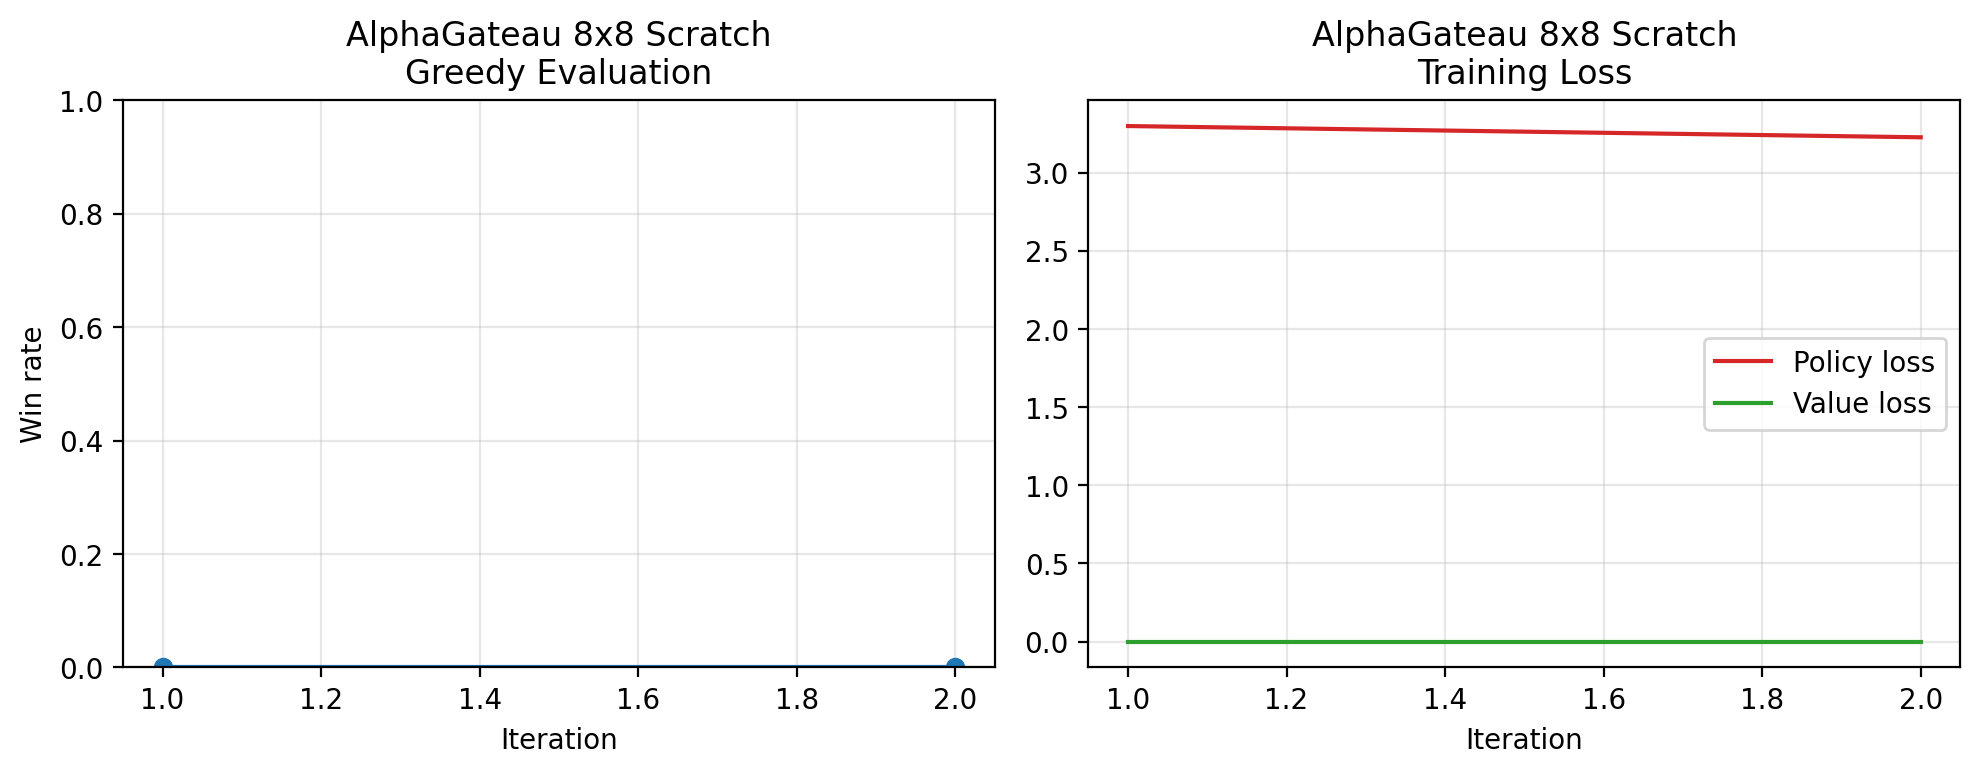
\includegraphics[width=\linewidth]{figures/gnn_8x8_scratch_curve.png}
  \caption{Smoke-generated 8x8 AlphaGateau scratch training curve.}
  \label{fig:scratch}
\end{figure}

\begin{figure}[t]
  \centering
  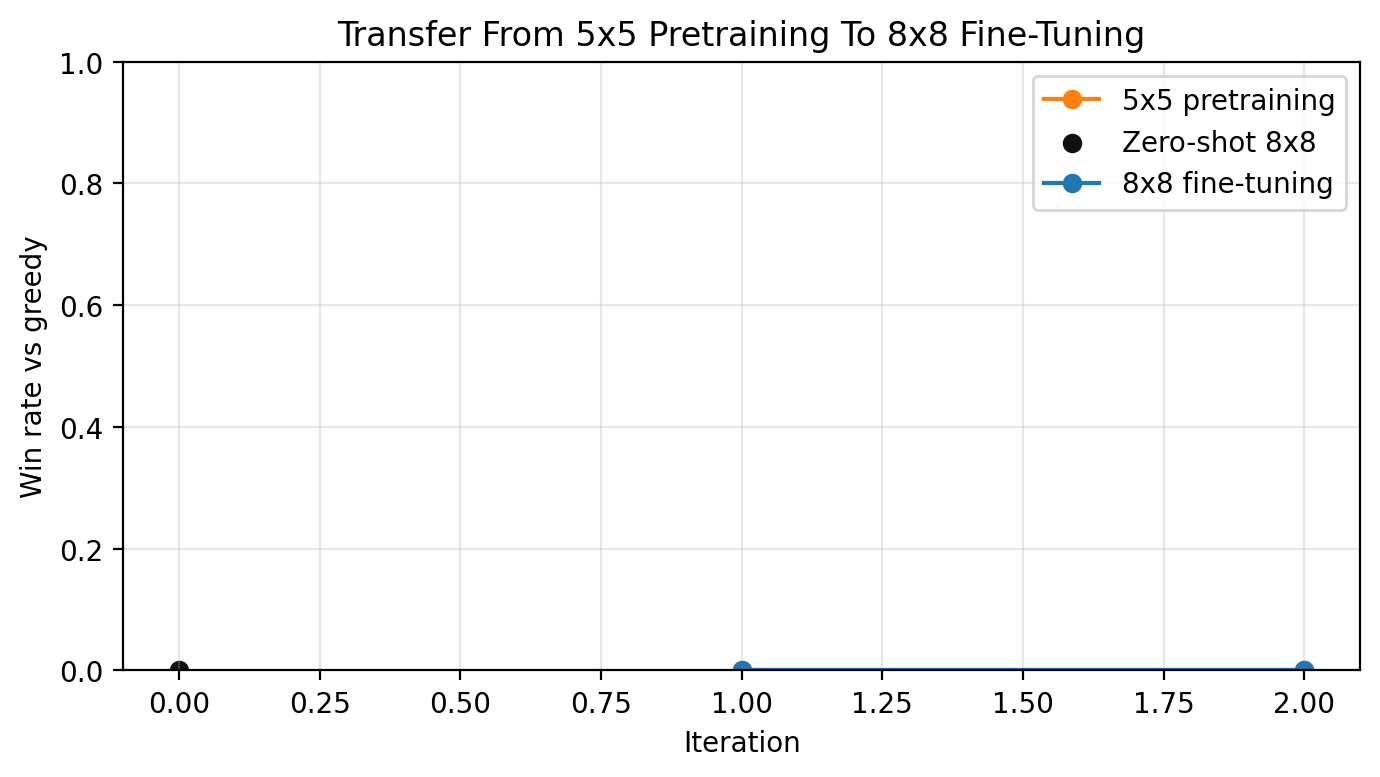
\includegraphics[width=\linewidth]{figures/transfer_curve.png}
  \caption{Smoke-generated transfer curve for 5x5 pretraining and 8x8 fine-tuning.}
  \label{fig:transfer}
\end{figure}

\begin{figure}[t]
  \centering
  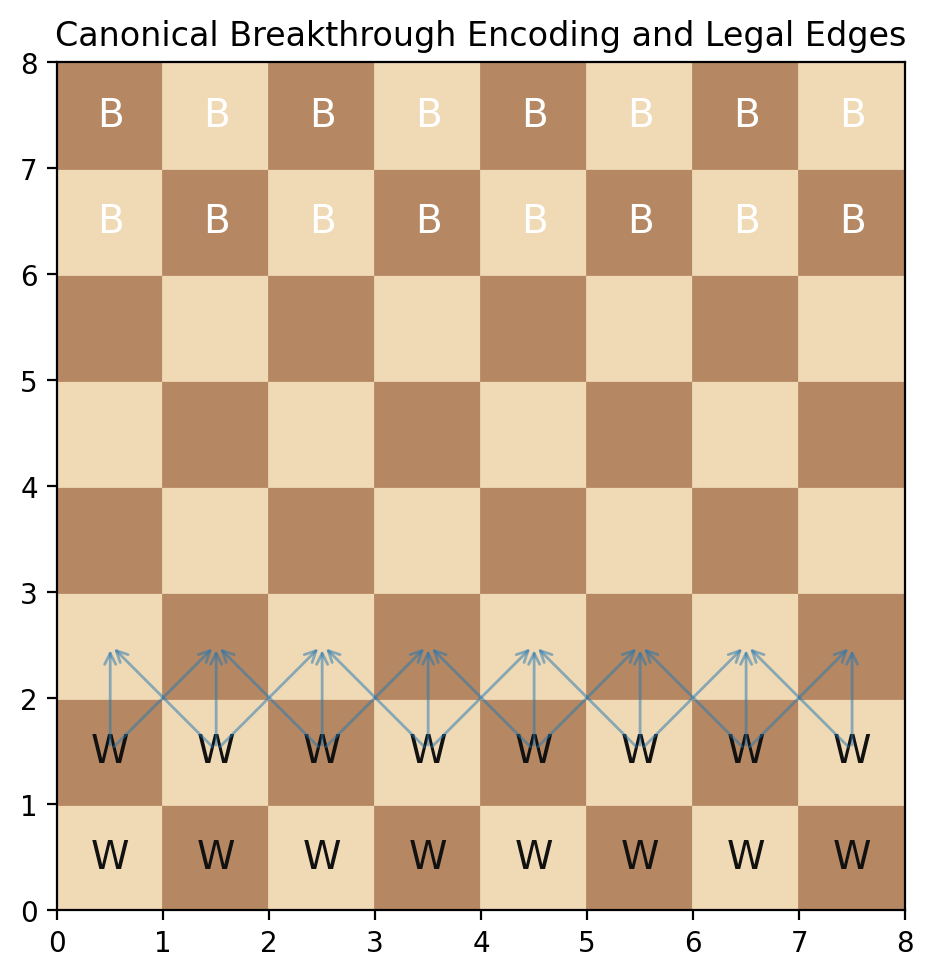
\includegraphics[width=0.72\linewidth]{figures/encoding_visualisation.png}
  \caption{Canonical Breakthrough encoding and legal-edge visualization.}
  \label{fig:encoding}
\end{figure}

These figures are designed to summarize both learning dynamics and the board/graph encoding used by the model. In a final course run, the 40/40/30/40-iteration schedule should be executed through the Slurm submitter before exporting the final PDF, but the smoke-generated figures already validate the reporting pipeline end-to-end.

\section{Discussion}

The main engineering result of this project is that AlphaGateau's graph formulation transfers cleanly to Breakthrough once the environment and graph-builder assumptions are decoupled from chess. The GNN path is genuinely board-size invariant: only the number of nodes and edges changes, while the feature schema and learned parameters remain fixed. This makes the 5x5-to-8x8 transfer experiment well-defined in a way that the CNN baseline is not.

The main practical tradeoff is compute. Even with a course-feasible schedule, self-play search dominates runtime. For that reason, the repository includes both smoke-scale commands for quick validation and a Slurm-native execution path for the actual project experiments, including retry chains that resume from saved training state across the 12-hour QoS boundary.

\section{Conclusion and Future Work}

We implemented a complete AlphaGateau-style Breakthrough project with a custom JAX environment, graph encoder, MCTS training loop, 8x8 CNN baseline, Elo evaluation, submission assets, and a reproducible Slurm workflow for the department GPUs. The central hypothesis remains that graph structure should improve both 8x8 learning efficiency and 5x5-to-8x8 transfer relative to a simpler grid baseline. The code now supports a clean empirical test of that hypothesis.

Natural next steps include larger runs, stronger search budgets, heuristic or handcrafted baselines, curriculum variants beyond 5x5, and ablations on edge features or attention pooling. A particularly useful follow-up would be to compare transfer from 5x5 pretraining against same-budget 8x8 scratch training under matched wall-clock limits.

\section{Contributions and Acknowledgements}

\textbf{Contributions.} Athmane Benarous: environment, training pipeline, and report integration. Farooq Khan: baseline experiments, analysis, and presentation material. Andrew Saffar: graph encoding, evaluation pipeline, and writeup support. These role assignments are placeholders and should be updated to match the final division of labor before submission.

\textbf{Acknowledgements.} We build on the public AlphaGateau chess implementation as an architectural reference and on JAX, Flax, Optax, Jraph, and MCTX for the underlying RL and GNN stack.

\begin{thebibliography}{9}

\bibitem{alphagateau}
A. Kulenkampff.
\newblock Enhancing Chess Reinforcement Learning with Graph Representation (AlphaGateau).
\newblock 2024.

\bibitem{breakthrough}
Breakthrough rules overview.
\newblock \url{https://en.wikipedia.org/wiki/Breakthrough_(board_game)}.

\bibitem{gat}
P. Veli\v{c}kovi\'{c} et al.
\newblock Graph Attention Networks.
\newblock 2017.

\bibitem{alphazero}
D. Silver et al.
\newblock A General Reinforcement Learning Algorithm that Masters Chess, Shogi, and Go through Self-Play.
\newblock 2017.

\bibitem{muzero}
D. Silver et al.
\newblock Mastering Atari, Go, Chess and Shogi by Planning with a Learned Model.
\newblock 2019.

\bibitem{repo}
AlphaGateau repository.
\newblock \url{https://github.com/akulen/AlphaGateau}.

\end{thebibliography}

\end{document}
